% !TeX spellcheck = en_GB
\subsubsection{Noise resistance}
Besides the efficiency of the networks the resistance of their predictions to noise is also of interest.
We create a noisy sequence $\{\ket{\phi_j}\}$ of N qubits from $\{\ket{\psi_j}\}$ using
\begin{align*}
	\ket{\phi_j} = e^{-i H_j \tau} \ket{\psi_j}, \ \forall j \in [1, N].
\end{align*}
$H_j$ are randomly generated Hermitian matrices and $\tau$ is a real parameter used to control the strength of the noise.
To quantify the dissimilarity between $\{\ket{\phi_j}\}$ and $\{\ket{\psi_j}\}$ we use the fidelity $F$ as defined in \cite{10.5555/1972505}:
\begin{align*}
	F_{\text{run}}(\{\ket{\phi_j}\}, \{\ket{\psi_j}\}) = \prod_j F(\ket{\phi_j}, \ket{\psi_j}) = \prod_j \abs{\bra{\phi_j}\ket{\psi_j}}.
\end{align*}

\begin{figure}
	\centering
	\begin{subfigure}{0.4\textwidth}
		\centering
		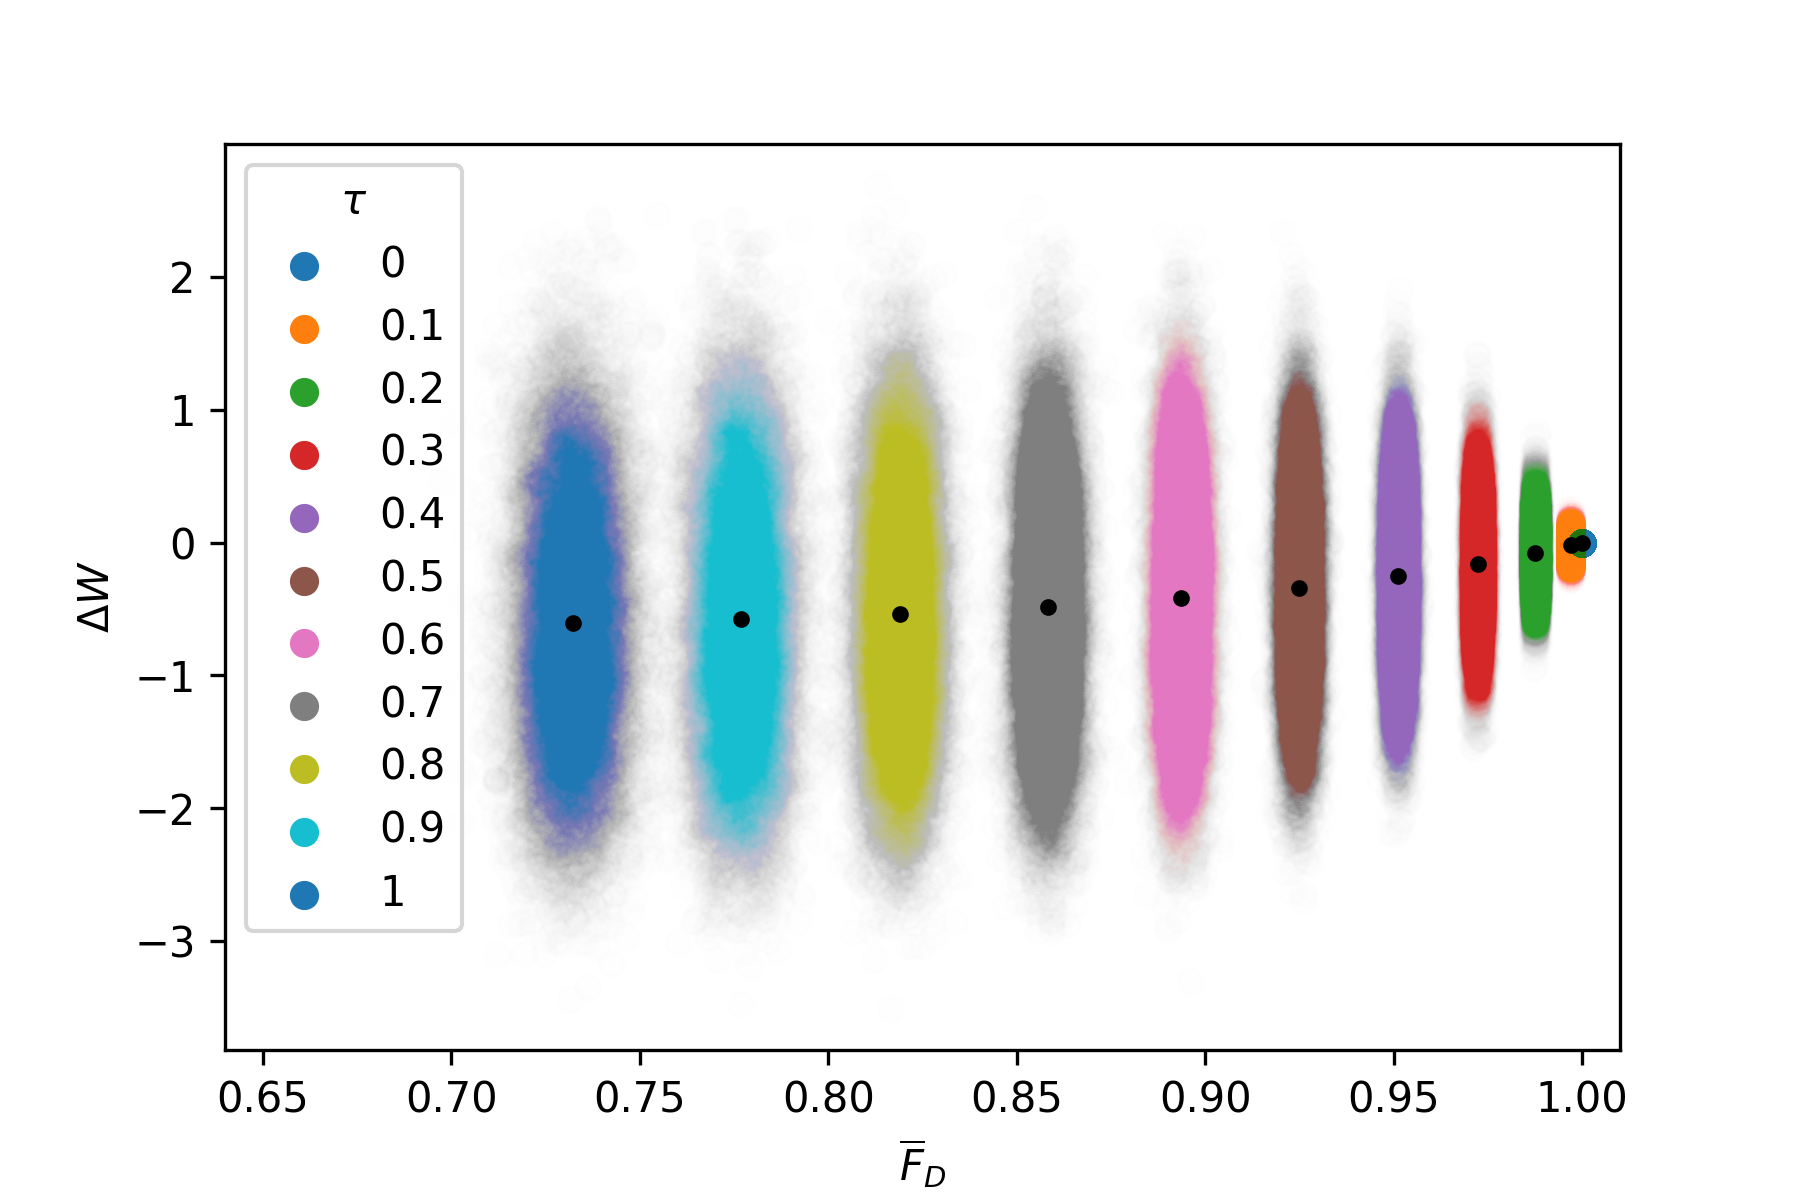
\includegraphics[width=\textwidth]{img/noisy_drive_bi_true_3}
		\subcaption{}
	\end{subfigure}
	\begin{subfigure}{0.4\textwidth}
		\centering
		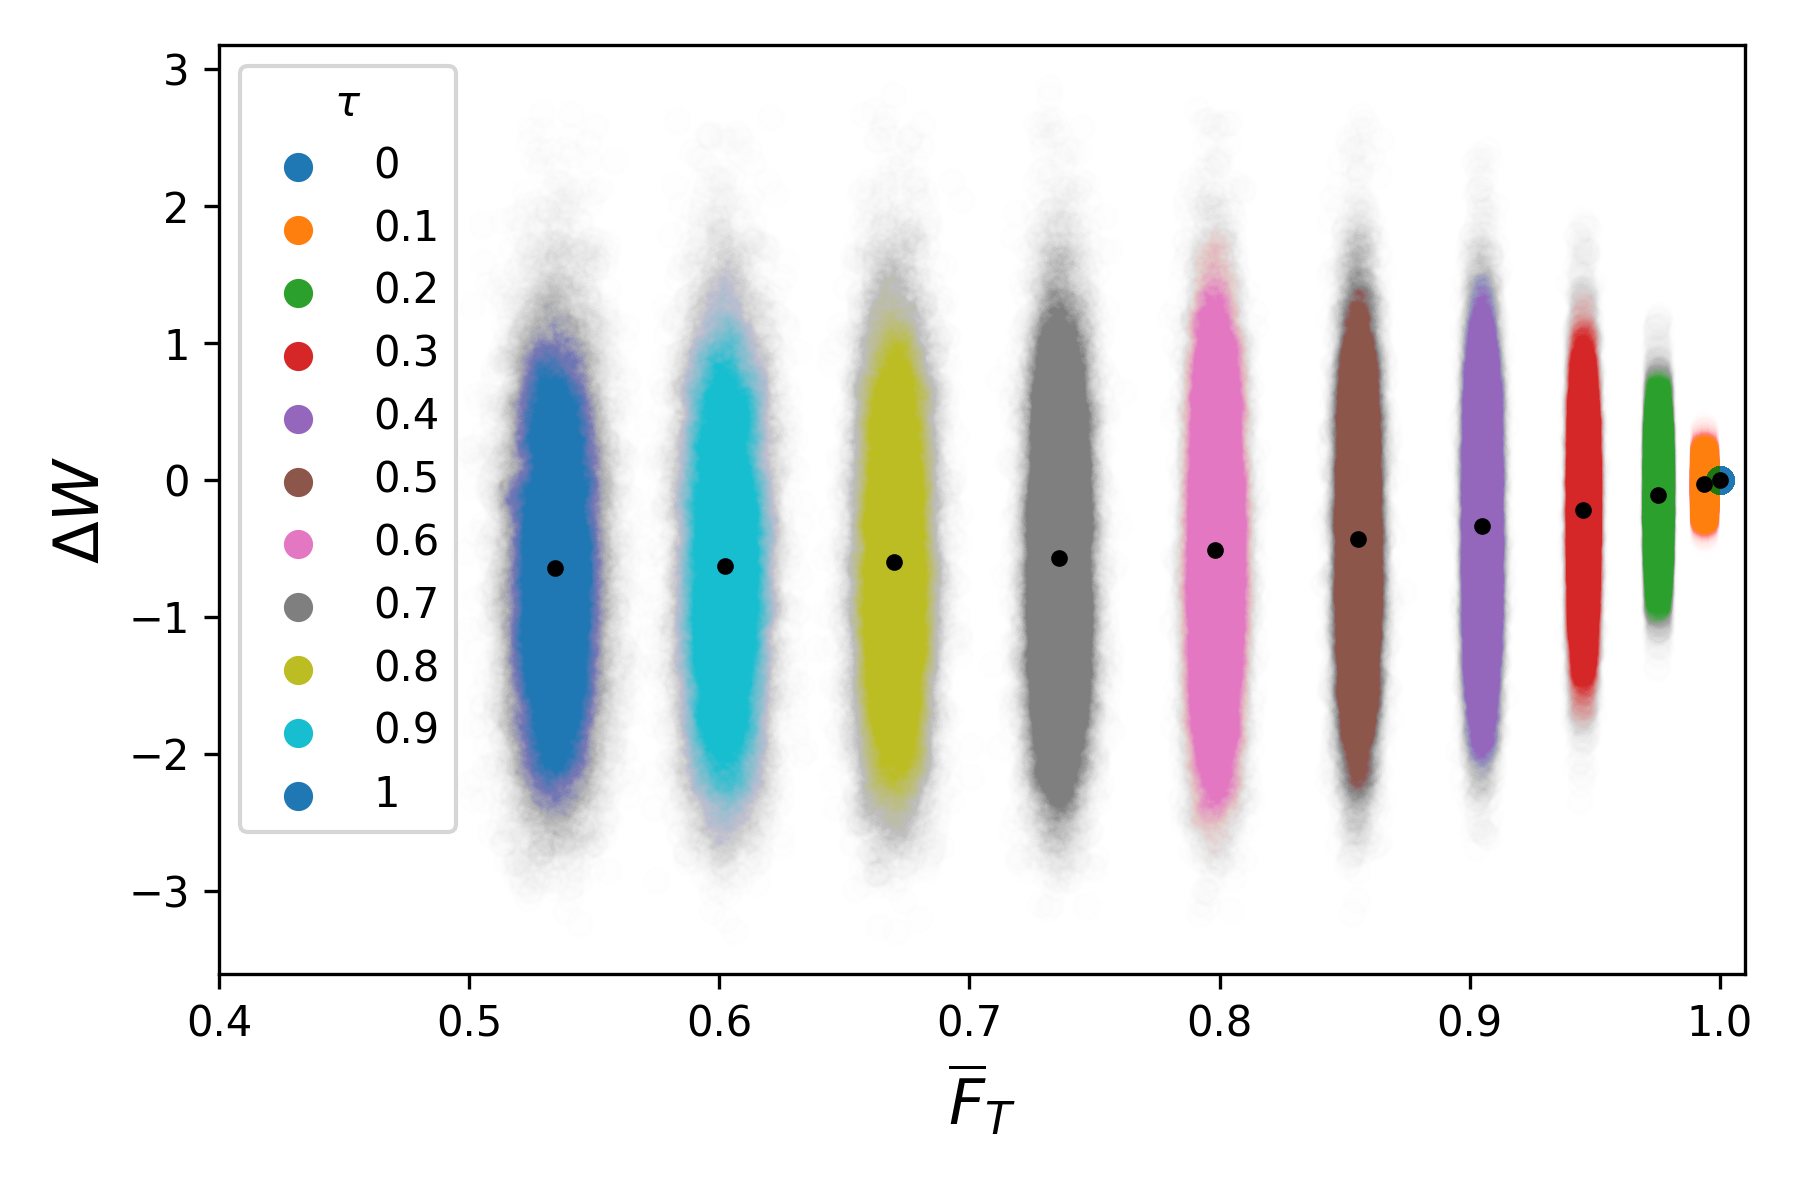
\includegraphics[width=\textwidth]{img/noisy_trans_bi_true_3}
		\subcaption{}
	\end{subfigure}
	\caption{We plot the difference $\Delta W = \overline{W}_{noise} - W_{pred}$ for the bidirectional LSTM. In (a), we create 100 noisy drive sequences }
\end{figure}